\section{Integer Linear Programming}

Integer Linear Program (ILP): $max\{c^Tx:x \in P  \cap Z^n\}$ with $P = \{x \in R^n : Ax \leq b\}$ \\
\textit{All variables are integer}

\begin{figure}[H]
\centering
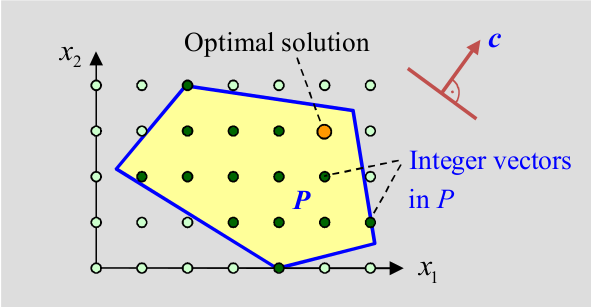
\includegraphics[width=0.4\textwidth]{figures/integerlp.png}
\caption{ILP}
\end{figure}

Mixed Integer LP (MIP): $max\{c^T x:x\in P \cap Z_K^n\}$ with $P = \{x \in R^n : Ax \leq b\}$ where $K  \subseteq \{1, ..., n\}$ and $Z_K^n = \{x \in R^n : x_j \in Z$ for $j \in K\}$ \\
\textit{Some variables are integer, others are not}

\begin{figure}[H]
\centering
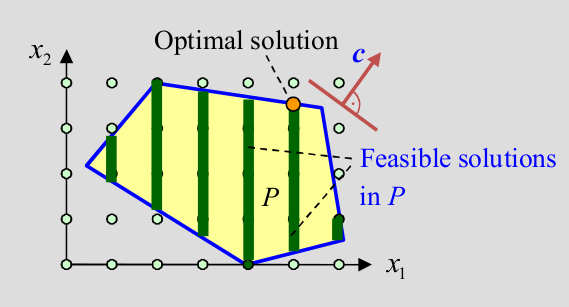
\includegraphics[width=0.4\textwidth]{figures/mlp.png}
\caption{MIP}
\end{figure}

It is not possible to just run a linear programming algorithm and then round the result up or down. 
\begin{itemize}
    \item Problem 1: Rounding the LP Solution may yield a non-feasible solution.
    \item Problem 2: The optimal LP Solution is maybe far away from the optimal ILP solution.
\end{itemize}

\clearpage

\subsection{Relaxations}

\begin{figure}[H]
\centering
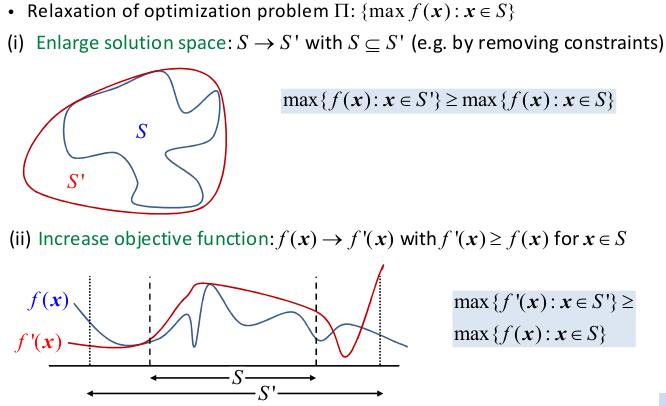
\includegraphics[width=0.5\textwidth]{figures/relaxations.png}
\caption{Relaxations}
\end{figure}

$\Rightarrow f'(x)$ need to be higher or equal to $f(x)$ within the solution space.

\subsection{Branch and Bound Method}
Branch-and-Bound (B\&B) is a general solution method (independent from ILP). 

Basic Procedure
\begin{enumerate}
    \item Split solution space iteratively into smaller subspaces ("Branch"). In each subproblem:
    \item Calculate an upper bound ("Bound") e.g. through relaxation
    \item Calculate a feasible solution $\Rightarrow$ Lower Bound ("Bound").
    \item Then use this information to "cut away" ("prune") certain subproblems.
\end{enumerate}

\clearpage
\subsubsection{Himmalaya Example}

\begin{itemize}
    \item We seperate the full solution space in several subspaces
    \item We send some helicopters to find the upper bound of these subspaces
    \item From the bottom, there are searching some sherpas for the lower bound
    \item At the end, we compare the values we got from each subspace.
\end{itemize}

\begin{figure}[H]
\centering
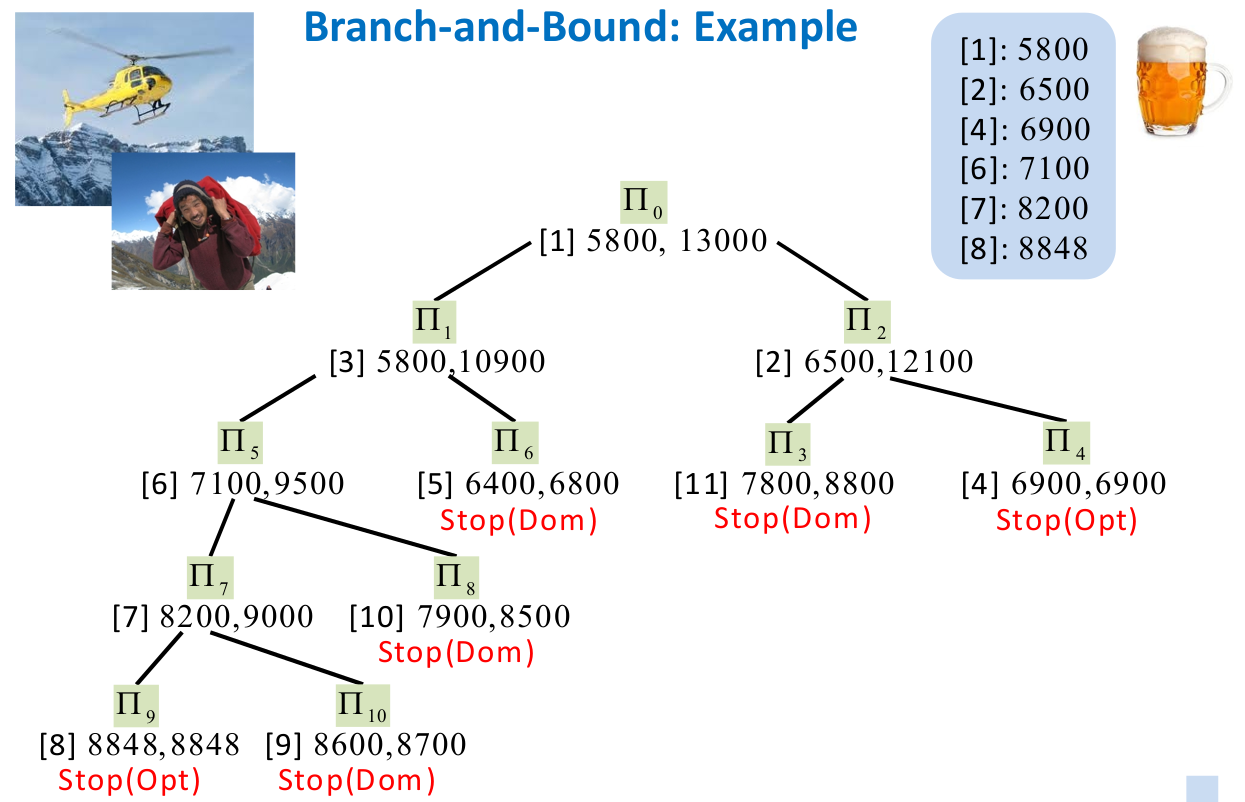
\includegraphics[width=0.8\textwidth]{figures/himmalayaExample.png}
\caption{Branch and Bound - Himmalaya Example}
\end{figure}

\begin{itemize}
    \item Stopping by Dominance means, that the upper bound is already lower than an already found maximum in the queue.
    \item Stopping by Optimum means, that we found the optimum in this area (upper and lower bound are the same).
\end{itemize}

\clearpage
\subsubsection{Knap-Sack Problem Example}

\begin{itemize}
    \item Items $j \in J$ have a volume $a_j$ and a benefit $c_j$.
    \item The knapsack has a capacity of $b$
    \item $max\{c^Tx:a^Tx\leq b, x \in \{0,1\}^j\}$
\end{itemize}
LP Solution easy:
\begin{enumerate}
    \item Sort the items by decreasing benefit per volume $\frac{c_j}{a_j}$
    \item Choose items in this order, until the knapsack is full. The last item fractionally. 
    \item After doing this, create two new branches. One branch with $x = 0$ for the fractional item and one branch with $x = 1$ for the fractional item. Continue until you discovered all options. 
\end{enumerate}

\begin{figure}[H]
\centering
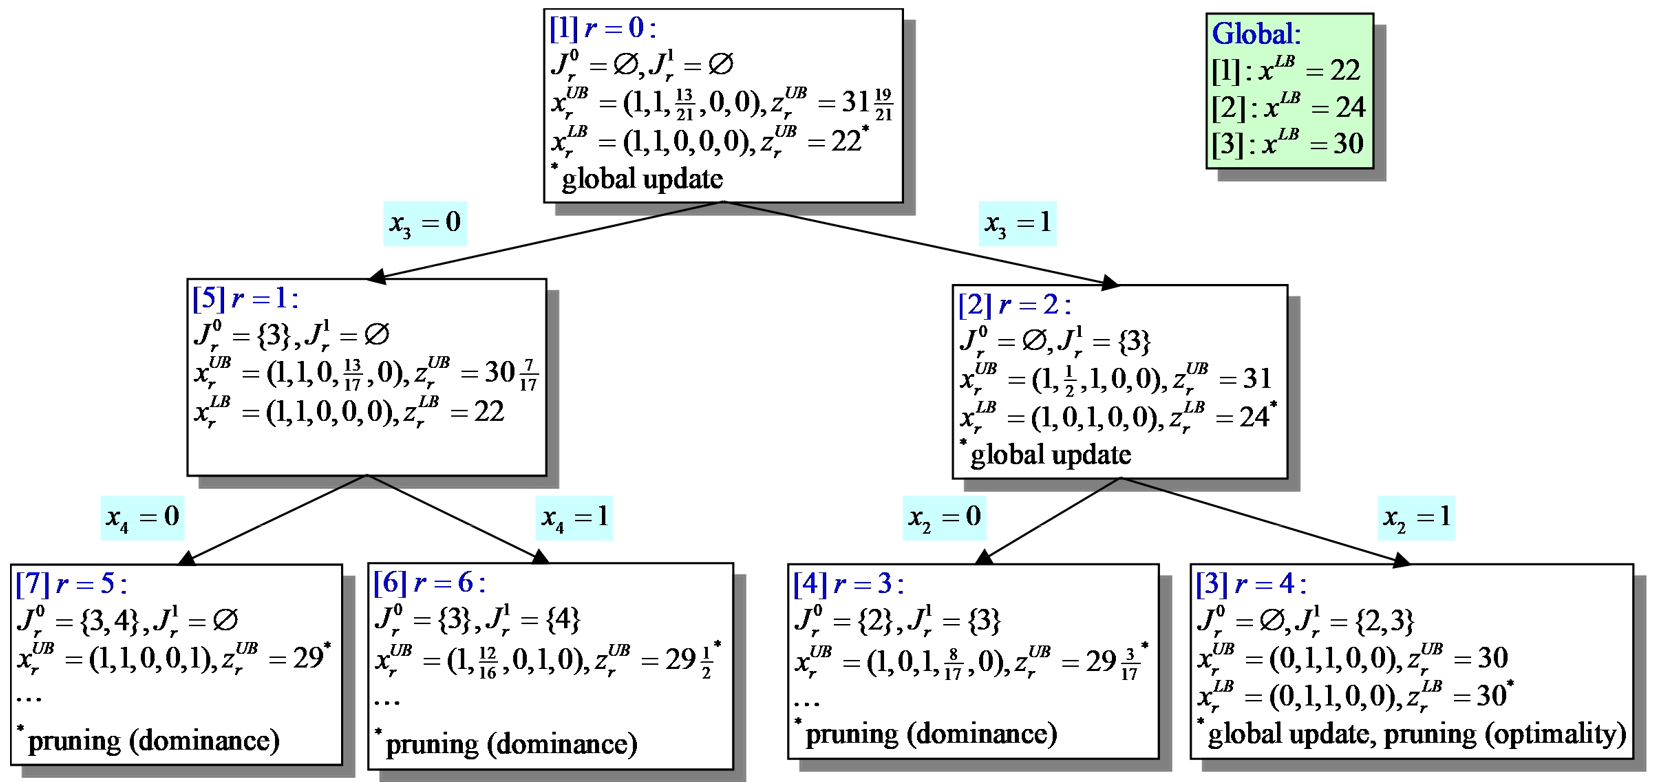
\includegraphics[width=1\textwidth]{figures/bbknapsack.png}
\caption{Branch and Bound - Knapsack Example}
\end{figure}

\clearpage

\subsection{Cutting Plane Method}

\begin{itemize}
    \item Let $P$ and $P'$ be two formulations for the ILP: $max\{c^Tx:x\in P \subseteq Z^n\}$. $P'$ is called a better solution is $P' \subseteq P$.
    \item And if $P' \subseteq P$ then $max\{c^Tx:x \in P'\} \leq max\{c^Tx:x \in P\}$
\end{itemize}


\begin{figure}[H]
\centering
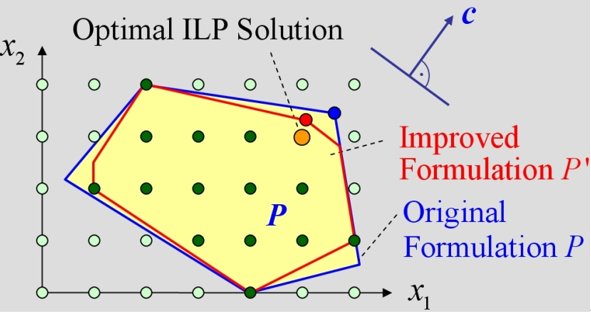
\includegraphics[width=0.4\textwidth]{figures/optimalilpsolution.png}
\caption{Cutting Plane Method - Optimal ILP Solution}
\end{figure}

\textbf{The best formulation for $P'$} would be the convex hull, which is the thightest polyhedrun around $P$, but this is nearly impossible to find. 

\begin{figure}[H]
\centering
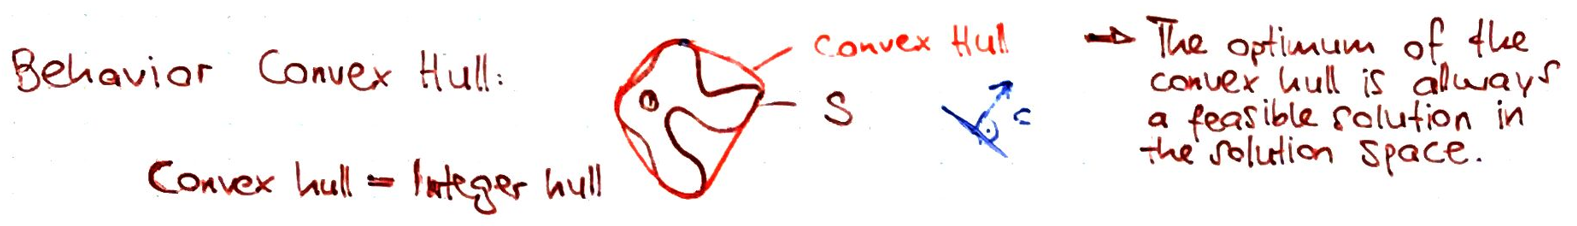
\includegraphics[width=0.8\textwidth]{figures/convexhull.png}
\caption{Cutting Plane Method - Behavior Convex Hull}
\end{figure}

\textbf{The integer hull of a polyhedrun is the convex hull, but only with integers.}

\begin{figure}[H]
\centering
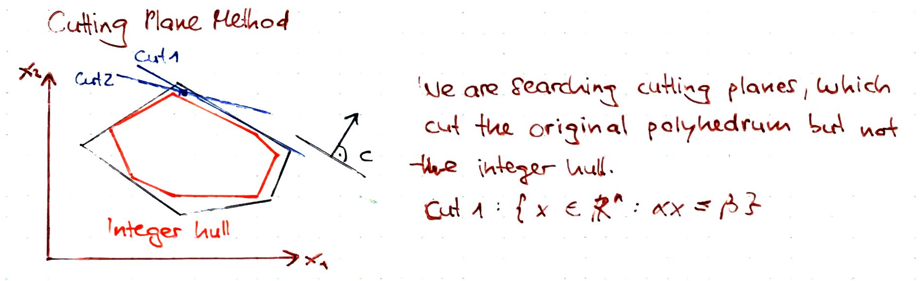
\includegraphics[width=1\textwidth]{figures/cuttingplanemethod.png}
\caption{Cutting Plane Method}
\end{figure}

\subsubsection{Gomory-Chvatal-Cut}

\begin{figure}[H]
\centering
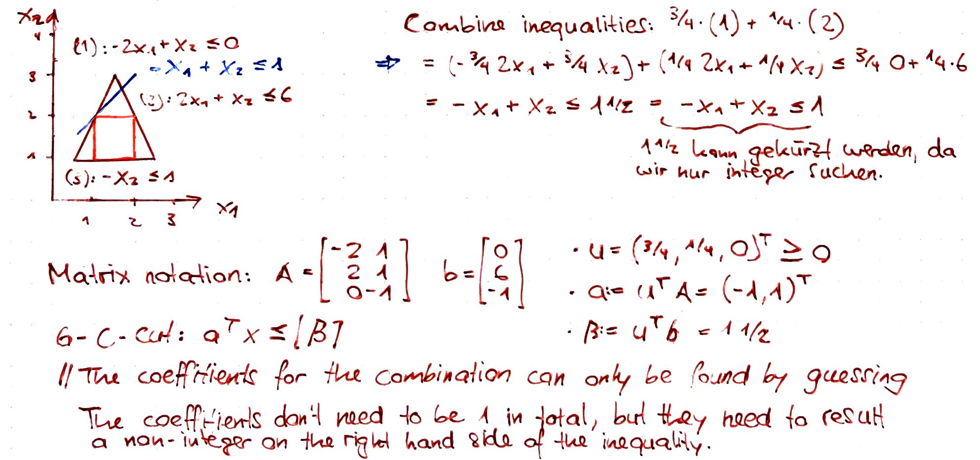
\includegraphics[width=1\textwidth]{figures/gomory.png}
\caption{Gomory-Chvatal-Cut}
\end{figure}

\clearpage